\documentclass[oneside]{article}


\author{Philipp Jetzlaff}
\title{Projektdokumentation}

%packages
\usepackage{fancyhdr}
\usepackage{graphicx}
\usepackage[a4paper, headheight=55pt, bottom=20mm]{geometry}
%Define Header
\fancyhf{}
\fancyhead[R]{
\includegraphics[width=0.11\textwidth]{OktoPOS.png}}
\fancyhead[L]{
  \uppercase{Erweiterung eines Onlineserivce}\\
  \vspace{1pt}
  \small{Anbindung der OktoPOS Software an den internen Übersetzungsdienst}\\ 
  \vspace{4pt}
  \scriptsize{\leftmark}
}
\fancyfoot[L]{Philipp Jetzlaff}
\fancyfoot[R]{\thepage}
\renewcommand{\headrulewidth}{1pt}
\renewcommand{\footrulewidth}{1pt}

%Define Codeblockfont
%Define imagepath
\graphicspath{{src/img/}}
\renewcommand{\listfigurename}{Abbildungsverzeichnis}
\renewcommand{\contentsname}{Inhaltsverzeichnis}
\begin{document}
%Define Header and footer
  \pagestyle{fancy}
  
  %Deckblatt einfügen
  %table of contents
  \pagenumbering{roman}
  \tableofcontents
  \addcontentsline{toc}{section}{\listfigurename}
  \listoffigures
  \addcontentsline{toc}{section}{\listtablename}
  \listoftables
  \newpage
  \section{Verzeichnis der Listings}
  \newpage
  \section{Glossar}
  \newpage
  \pagenumbering{arabic}
  \section{Einleitung}
  \subsection{Projektbeschreibung}
  \subsection{Projektziel}
  \subsection{Projektumfeld}
  \subsection{Projektabgrenzung}
  \section{Projektplanung}
  \subsection{Projektphasen}
  \subsection{Vorgehensmodel}
  \subsection{Genutzte Resourcen}
  \section{Analysephase}
  \subsection{Ist-Analyse}
  \begin{figure}[h]
    \centering
    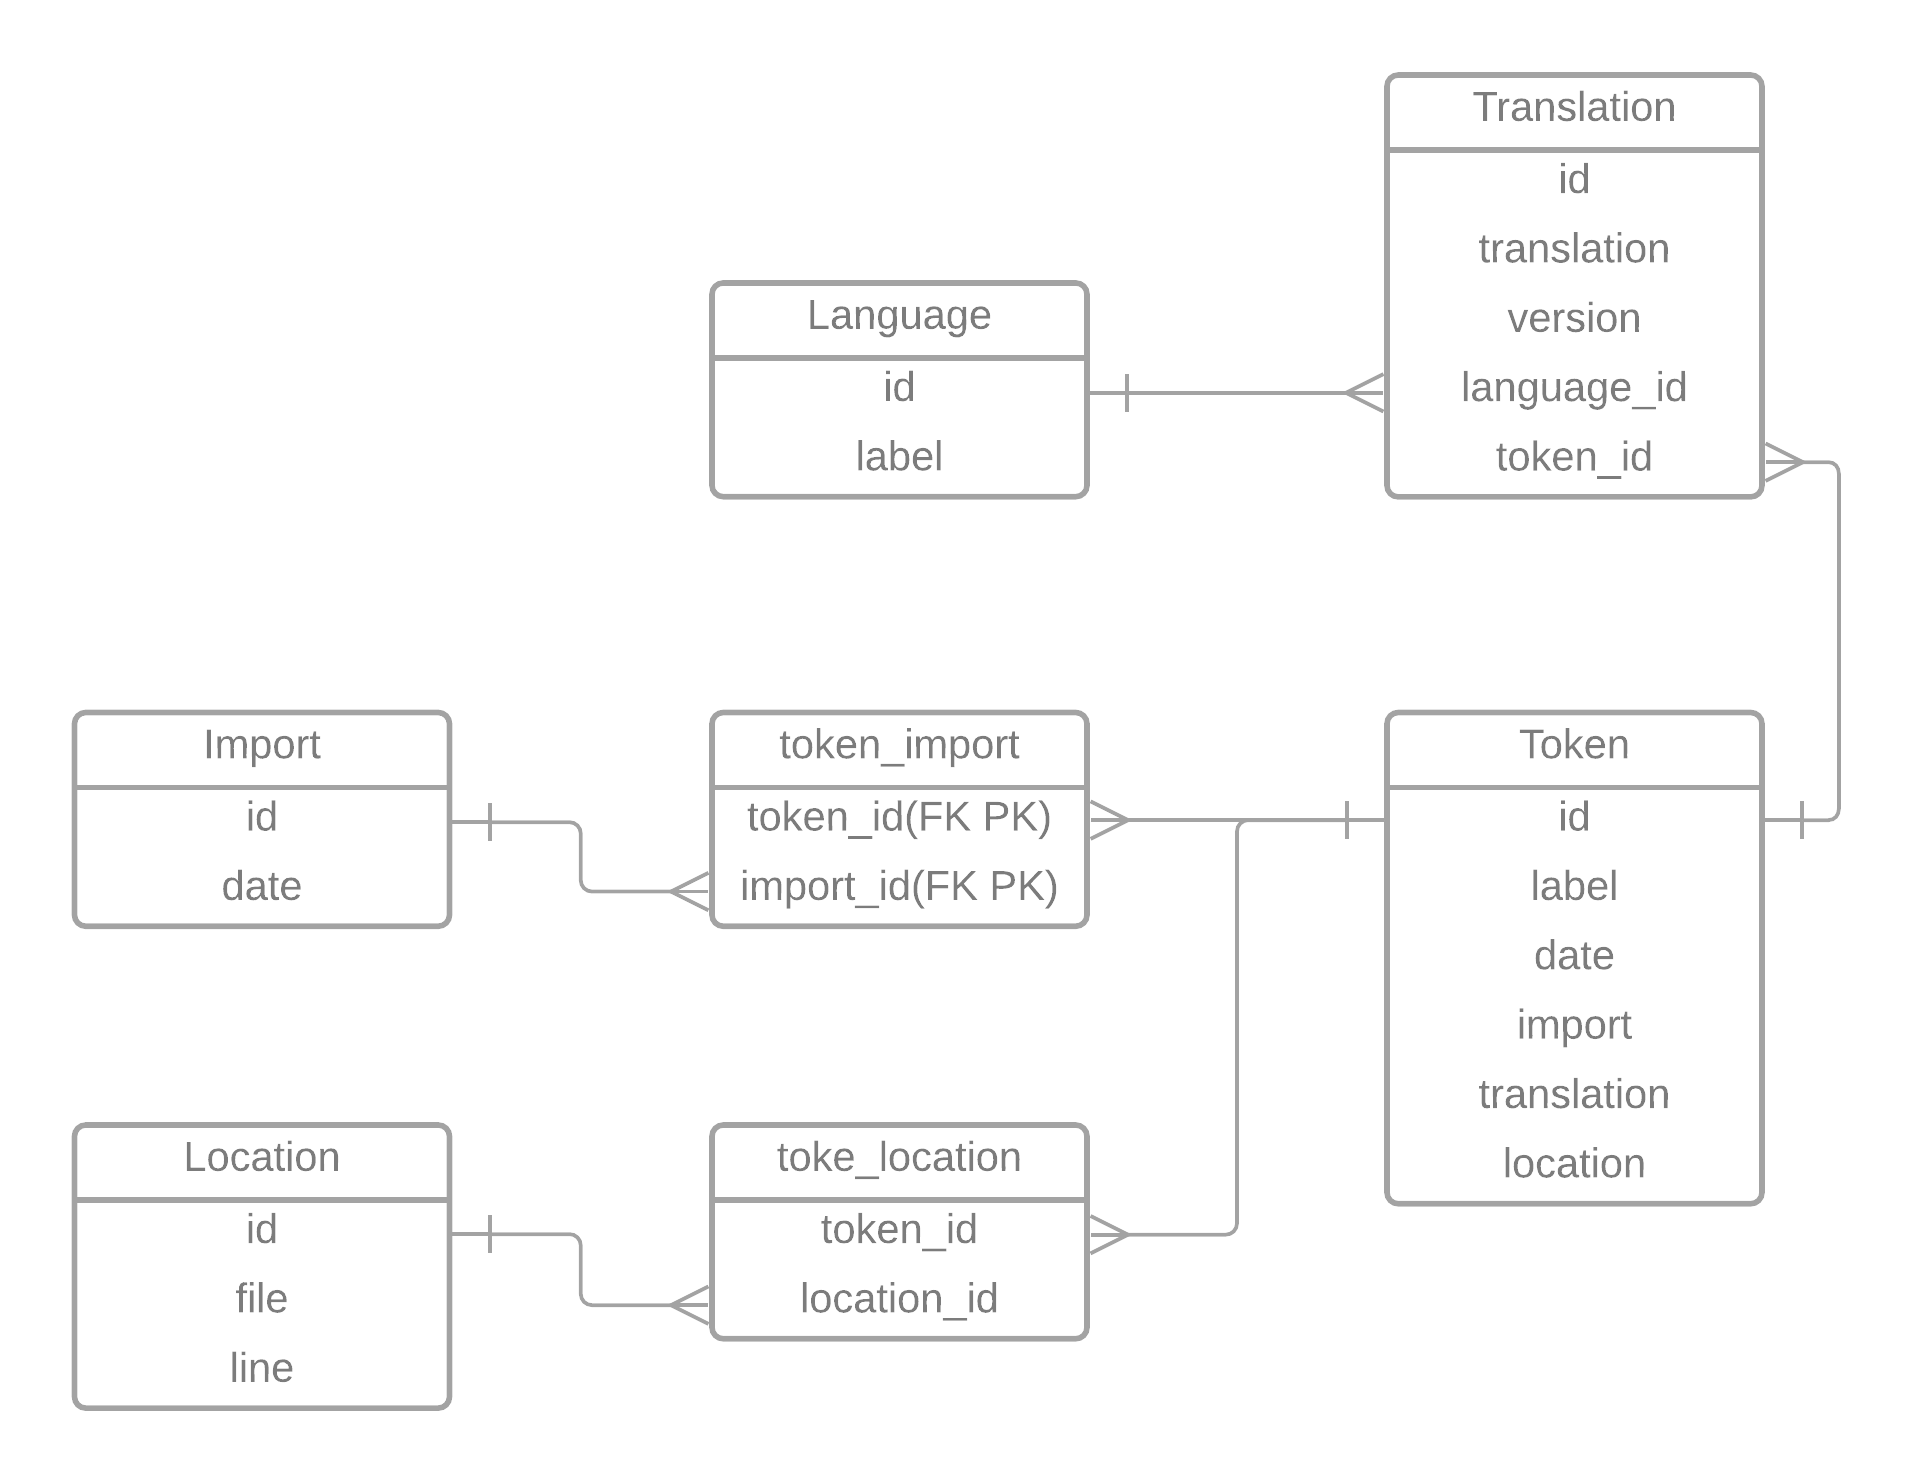
\includegraphics[width=\textwidth]{ERD_TranslationService_IST-Analyse.png}
    \caption{ERD im IST Zustand}
  \end{figure}
  \newpage
  \subsection{Soll-Analyse}
  asd
  \begin{figure}[h]
    \centering
    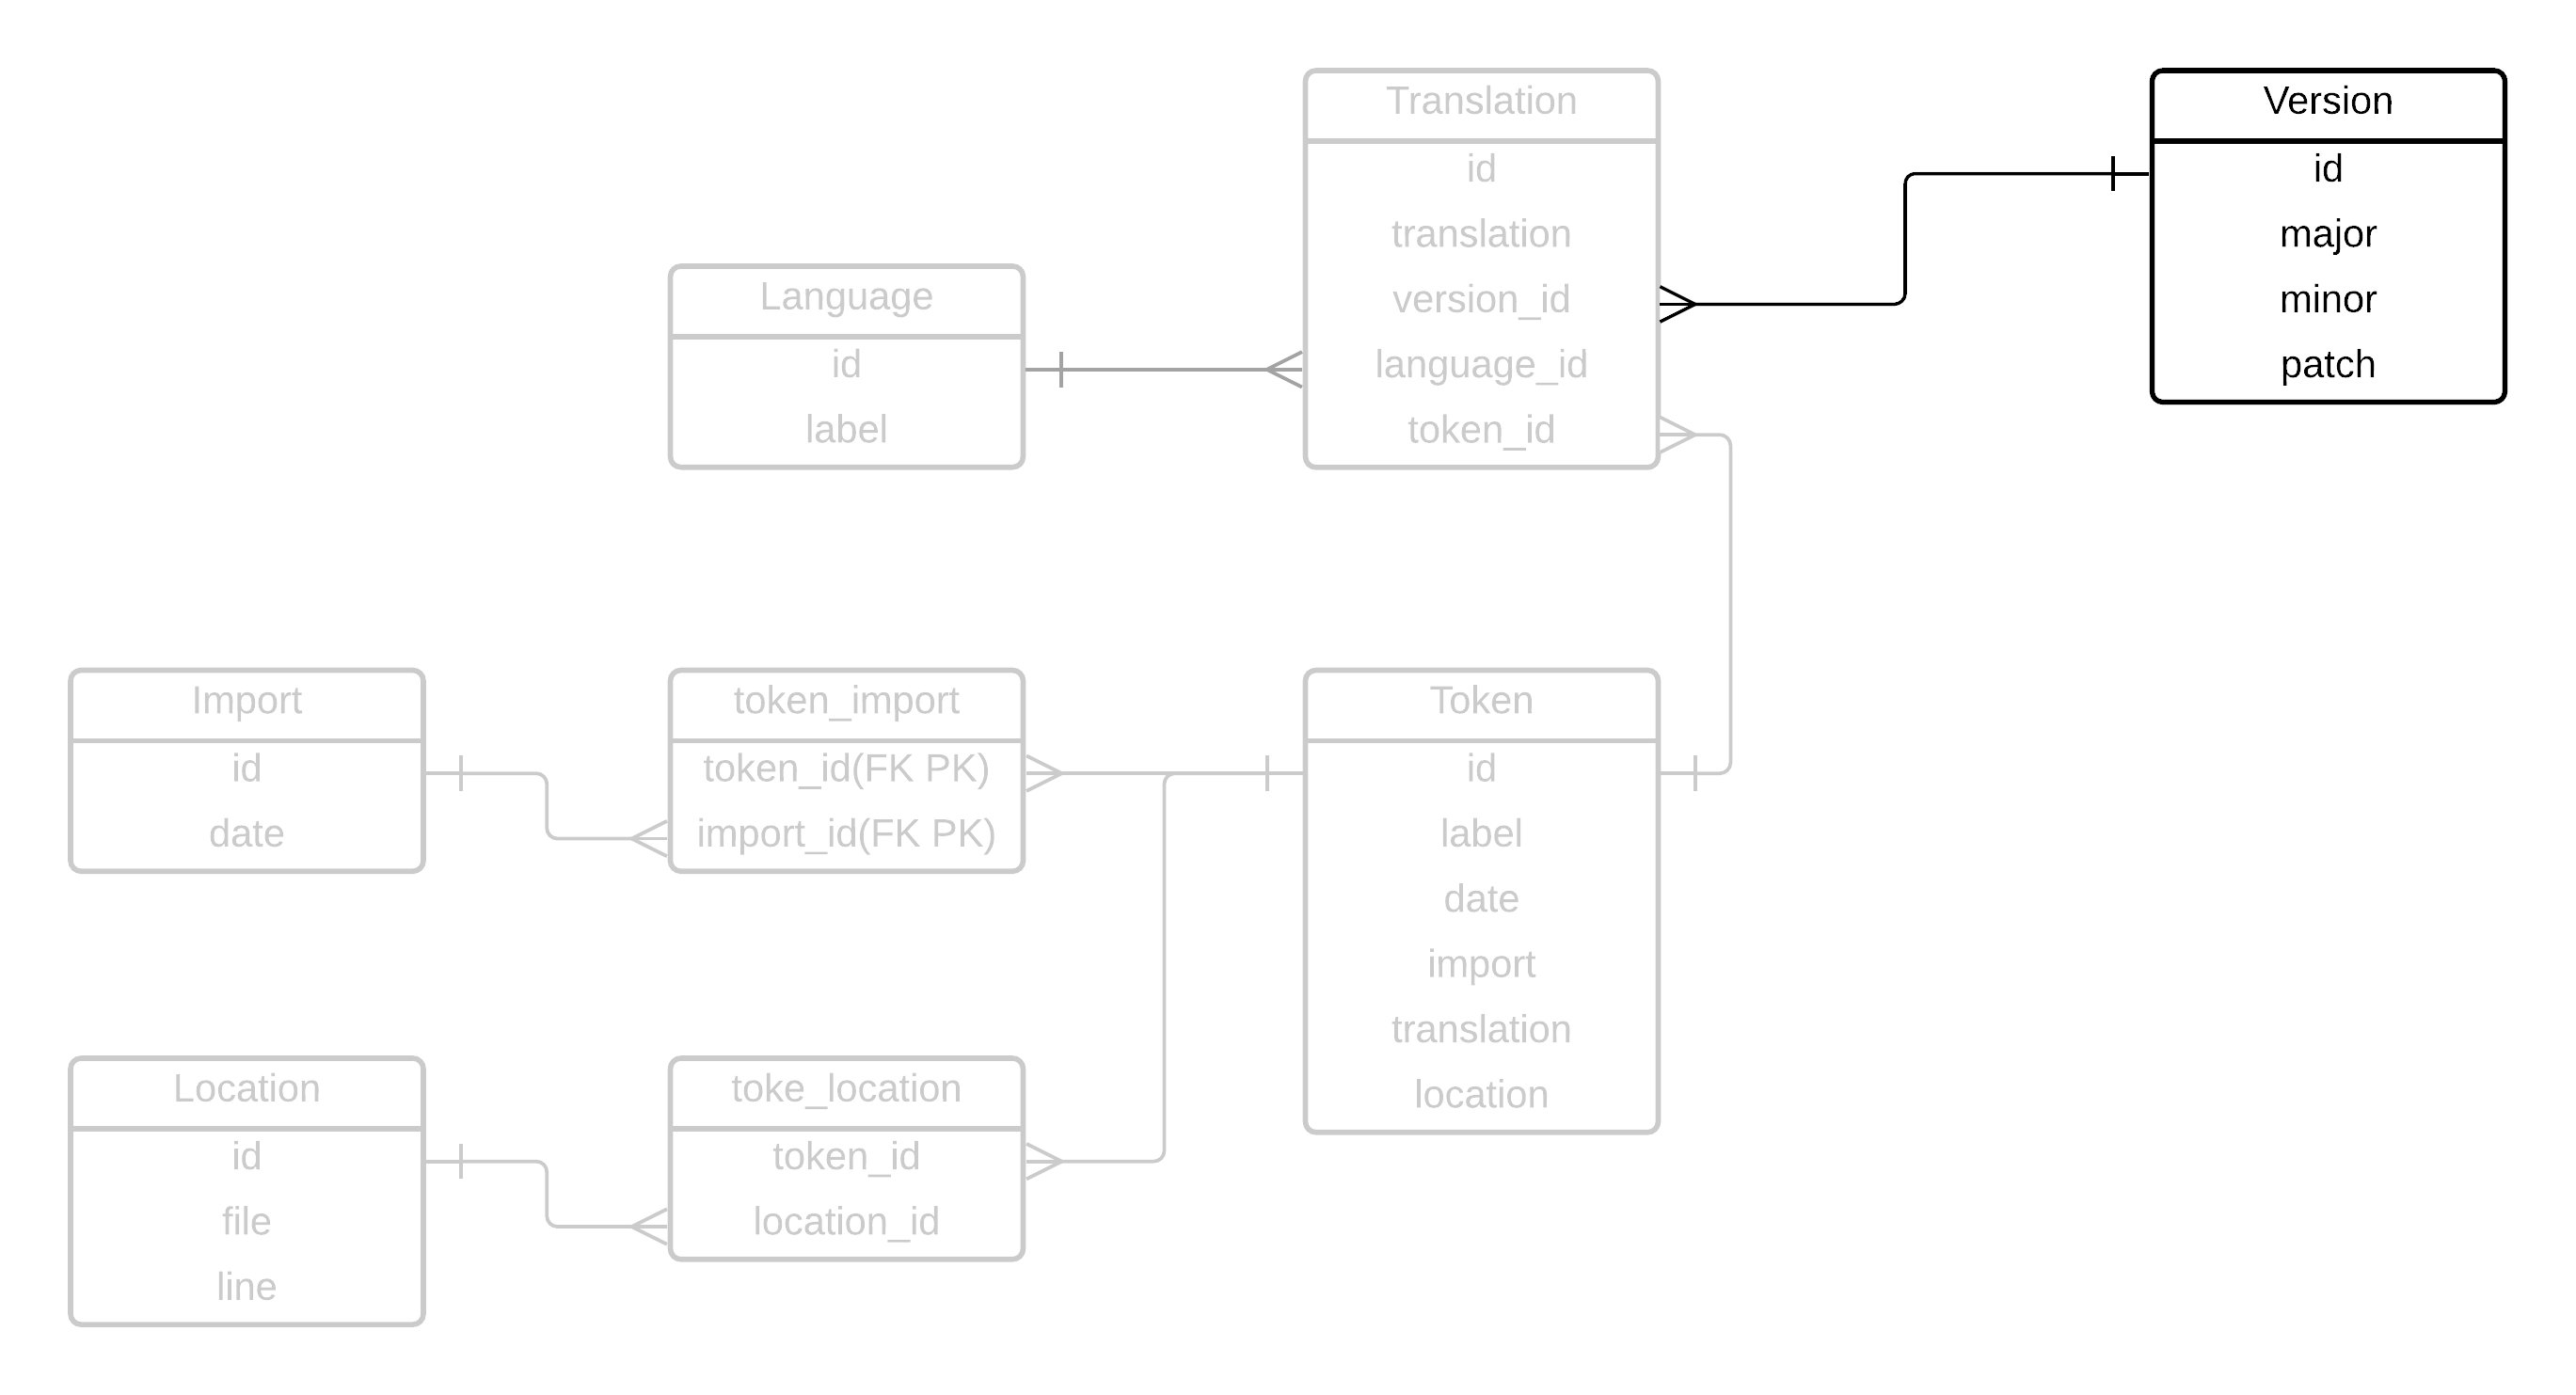
\includegraphics[width=\textwidth]{ERD_TranslationService_SOLL-Analyse.png}
    \caption{ERD im SOLL Zustand}
  \end{figure}  
  \subsection{Wirtschaftsanalyse}
  \subsubsection{Kostenaufstellung}
  \subsubsection{Aromatisierungsdauer}
  \subsection{Anwendungsfälle}
  \subsection{Lastenheft}
  \section{Entwurfsphase}
  \subsection{Userinterface}
  \subsection{Datenmodell}
  \subsection{APIs}
  \subsection{Geschäftslogik}
  \subsection{Testcases}
  \subsection{Pflichtenheft}
  \section{Implementierungsphase}
  \subsection{Translationservice}
  \subsubsection{Erweiterung der bestehenen Datengrundlage}
  \subsubsection{Implemetierung der REST Api}
  \subsection{Translationloader}
  \subsubsection{Geschäftslogik}
  \subsubsection{Userinterface}
  \subsubsection{Batch Script Extension}
  \subsubsection{Webhook}
  \section{Abnahme- und Einführungsphase}
  \subsection{Abnahme durch den Fachbereich}
  \subsection{Deployment}
  \section{Dokumentation}
  \section{Retroanalyse}
  \subsection{IST-SOLL-Vergleich}
  \subsection{Ausblick}
  \setcounter{section}{0}
  \renewcommand{\thesection}{\MakeUppercase{\alph{section}}}
  \section{Anhang}
  \subsection{Schnittstelledokumentation}
  Swagger
\end{document}